%	INTRODUZIONE


\subsection{Descrizione del Gioco}
	
	Touch the color, o "Strega chiama color" nella sua versione italiana, � un semplice gioco di gruppo da svolgersi all'aria aperta. Questo prevede la selezione di un giocatore del gruppo al ruolo di strega, il quale dovr� scegliere un colore ed urlarne il nome a tutti gli altri componenti del gruppo. Quest'ultimi, udito il colore, dovranno cercare nel minor tempo possibile un oggetto del colore indicatogli per poi raggiungerlo: perde l'ultimo giocatore a "toccare il colore" e verr� selezionato come strega al prossimo giro. 
	
	Nel resto della documentazione i robot nel ruolo della strega verranno chiamati nodi Witch e quelli nel ruolo del resto del gruppo verranno chiamati nodi Kid.
	
	\subsection{Nicchia Ecologica}
	Nella progettazione di un sistema robotico, al progettista devono essere chiare fin dal principio tre cose:
	\begin{itemize}
		\item il task, o i task, che il robot dovr� compiere;
		\item le caratteristiche del robot;
		\item le caratteristiche dell'ambiente in cui il robot agir�.
	\end{itemize}
	La definizione di queste tre cose specifica quella che si chiama \textit{nicchia ecologica} del robot. La nicchia ecologica permette di definire vincoli e potenzialit� del sistema.
	
	Per quanto riguarda il primo punto, il task, abbiamo delle differenze fra nodi Witch e nodi Kid. Per i primi si tratta di un task molto semplice, esso prevede nell'ordine:
	\begin{itemize}
		\item la scelta di un colore da un pool ben definito;
		\item la comunicazione del colore ai nodi Kid;
		\item la comunicazione della fine del gioco ai nodi Kid una volta ricevuto $n-1$ messaggi di "colore toccato", dove $n$ � il numero di nodi Kid.
	\end{itemize}
	Si tratta quindi, per i nodi Witch, di un task a tempo illimitato, robot-based, senza movimento e dipendente, in quanto la comunicazione della fine del gioco dipende da comunicazioni precedenti dei nodi Kid.
	Per i nodi Kid, invece, il task prevede:
	\begin{itemize}
		\item trovare un oggetto del colore comunicatogli e raggiungerlo;
		\item comunicare al nodo Witch che ha toccato il colore.
	\end{itemize}
	I nodi Kid quindi svolgono un task minimum-time, in quanto devono cercare di portare a termine il task nel minor tempo possibile, object-based, movement-to e dipendente, per motivazioni simili a quelle fatte per i nodi Witch.
	
	Per quanto riguarda i robot, si tratta di \textit{Pioneer} modello 3-DX munito di due ruote motrici fisse ed una mobile e dodici (o sei) sensori sonar. Sulla base superiore abbiamo installato una telecamera RGB-D (\textit{Microsoft Kinect}) la quale viene utilizzata per le funzioni di computer vision.
	
	Per quanto riguarda l'organizzazione dei robot, invece, abbiamo una composizione eterogenea (o omogenea in quanto si tratta dello stessod tipo di robot????), dalla grandezza limitata, la cui riconfigurabilit� � comunicata, avente comunicazione esplicita con topologia ad albero.

\subsection{Schema dei Behaviours}

	Come per il resto, lo schema dei behaviours si differenzia in base al tipo di nodo che consideriamo. La Figura~\ref{fig:stregabeh} mostra lo schema riferito ai nodi Witch, la Figura~\ref{fig:bambinobeh} quello riferito ai nodi Kid.
	
	% Figura 
	\begin{figure}[h]
		\centering
		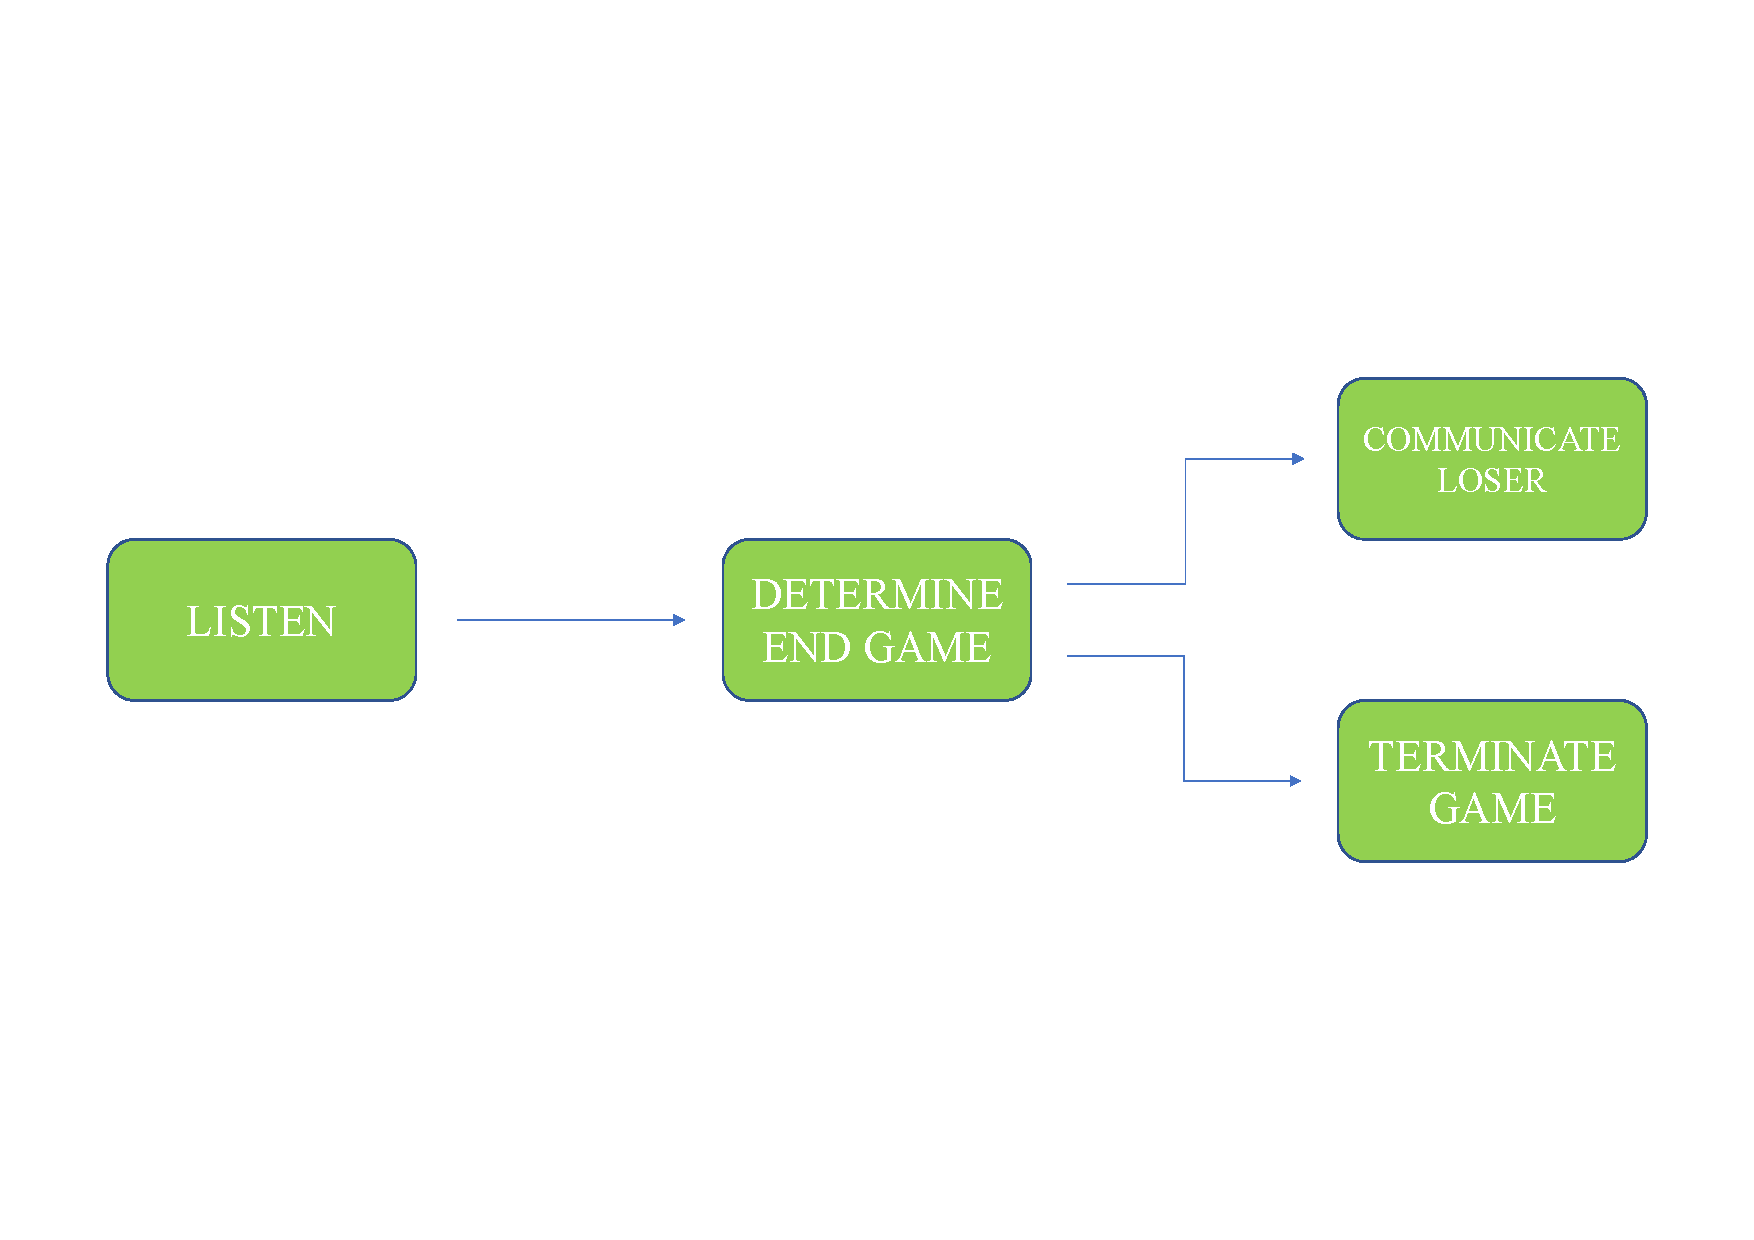
\includegraphics[width=0.9\textwidth]{images/stregabeh.pdf}
		\caption{Schema dei behaviours dei nodi Witch.}
		\label{fig:stregabeh}
	\end{figure}
	
	% Figura 
	\begin{figure}[h]
		\centering
		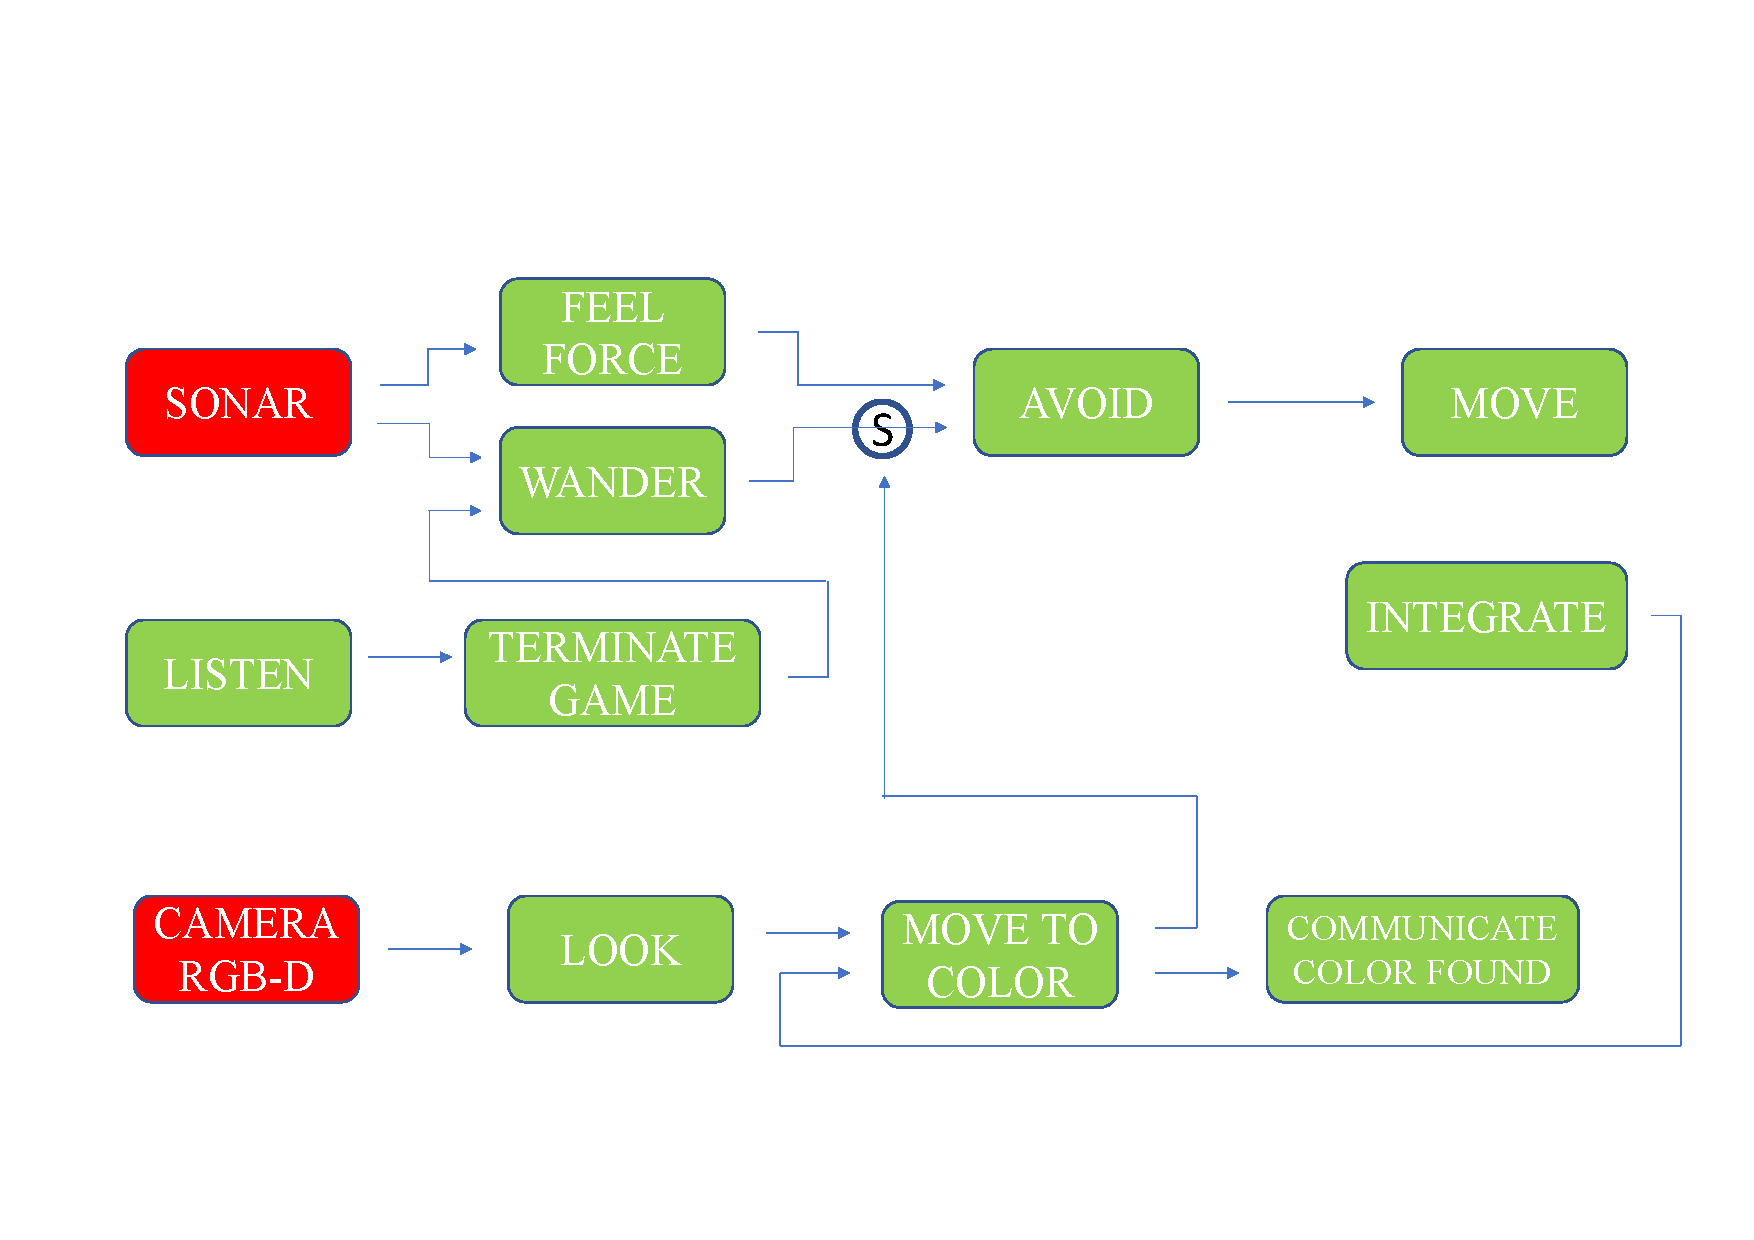
\includegraphics[width=0.9\textwidth]{images/bambinobeh.pdf}
		\caption{Schema dei behaviours dei nodi Kid.}
		\label{fig:bambinobeh}
	\end{figure}
